% Options for packages loaded elsewhere
\PassOptionsToPackage{unicode}{hyperref}
\PassOptionsToPackage{hyphens}{url}
%
\documentclass[
]{article}
\usepackage{amsmath,amssymb}
\usepackage{lmodern}
\usepackage{iftex}
\ifPDFTeX
  \usepackage[T1]{fontenc}
  \usepackage[utf8]{inputenc}
  \usepackage{textcomp} % provide euro and other symbols
\else % if luatex or xetex
  \usepackage{unicode-math}
  \defaultfontfeatures{Scale=MatchLowercase}
  \defaultfontfeatures[\rmfamily]{Ligatures=TeX,Scale=1}
\fi
% Use upquote if available, for straight quotes in verbatim environments
\IfFileExists{upquote.sty}{\usepackage{upquote}}{}
\IfFileExists{microtype.sty}{% use microtype if available
  \usepackage[]{microtype}
  \UseMicrotypeSet[protrusion]{basicmath} % disable protrusion for tt fonts
}{}
\makeatletter
\@ifundefined{KOMAClassName}{% if non-KOMA class
  \IfFileExists{parskip.sty}{%
    \usepackage{parskip}
  }{% else
    \setlength{\parindent}{0pt}
    \setlength{\parskip}{6pt plus 2pt minus 1pt}}
}{% if KOMA class
  \KOMAoptions{parskip=half}}
\makeatother
\usepackage{xcolor}
\IfFileExists{xurl.sty}{\usepackage{xurl}}{} % add URL line breaks if available
\IfFileExists{bookmark.sty}{\usepackage{bookmark}}{\usepackage{hyperref}}
\hypersetup{
  pdftitle={Transformer les fichiers du Ministère de l'Intérieur},
  pdfauthor={Frédérik Cassor},
  hidelinks,
  pdfcreator={LaTeX via pandoc}}
\urlstyle{same} % disable monospaced font for URLs
\usepackage[margin=1in]{geometry}
\usepackage{color}
\usepackage{fancyvrb}
\newcommand{\VerbBar}{|}
\newcommand{\VERB}{\Verb[commandchars=\\\{\}]}
\DefineVerbatimEnvironment{Highlighting}{Verbatim}{commandchars=\\\{\}}
% Add ',fontsize=\small' for more characters per line
\usepackage{framed}
\definecolor{shadecolor}{RGB}{248,248,248}
\newenvironment{Shaded}{\begin{snugshade}}{\end{snugshade}}
\newcommand{\AlertTok}[1]{\textcolor[rgb]{0.94,0.16,0.16}{#1}}
\newcommand{\AnnotationTok}[1]{\textcolor[rgb]{0.56,0.35,0.01}{\textbf{\textit{#1}}}}
\newcommand{\AttributeTok}[1]{\textcolor[rgb]{0.77,0.63,0.00}{#1}}
\newcommand{\BaseNTok}[1]{\textcolor[rgb]{0.00,0.00,0.81}{#1}}
\newcommand{\BuiltInTok}[1]{#1}
\newcommand{\CharTok}[1]{\textcolor[rgb]{0.31,0.60,0.02}{#1}}
\newcommand{\CommentTok}[1]{\textcolor[rgb]{0.56,0.35,0.01}{\textit{#1}}}
\newcommand{\CommentVarTok}[1]{\textcolor[rgb]{0.56,0.35,0.01}{\textbf{\textit{#1}}}}
\newcommand{\ConstantTok}[1]{\textcolor[rgb]{0.00,0.00,0.00}{#1}}
\newcommand{\ControlFlowTok}[1]{\textcolor[rgb]{0.13,0.29,0.53}{\textbf{#1}}}
\newcommand{\DataTypeTok}[1]{\textcolor[rgb]{0.13,0.29,0.53}{#1}}
\newcommand{\DecValTok}[1]{\textcolor[rgb]{0.00,0.00,0.81}{#1}}
\newcommand{\DocumentationTok}[1]{\textcolor[rgb]{0.56,0.35,0.01}{\textbf{\textit{#1}}}}
\newcommand{\ErrorTok}[1]{\textcolor[rgb]{0.64,0.00,0.00}{\textbf{#1}}}
\newcommand{\ExtensionTok}[1]{#1}
\newcommand{\FloatTok}[1]{\textcolor[rgb]{0.00,0.00,0.81}{#1}}
\newcommand{\FunctionTok}[1]{\textcolor[rgb]{0.00,0.00,0.00}{#1}}
\newcommand{\ImportTok}[1]{#1}
\newcommand{\InformationTok}[1]{\textcolor[rgb]{0.56,0.35,0.01}{\textbf{\textit{#1}}}}
\newcommand{\KeywordTok}[1]{\textcolor[rgb]{0.13,0.29,0.53}{\textbf{#1}}}
\newcommand{\NormalTok}[1]{#1}
\newcommand{\OperatorTok}[1]{\textcolor[rgb]{0.81,0.36,0.00}{\textbf{#1}}}
\newcommand{\OtherTok}[1]{\textcolor[rgb]{0.56,0.35,0.01}{#1}}
\newcommand{\PreprocessorTok}[1]{\textcolor[rgb]{0.56,0.35,0.01}{\textit{#1}}}
\newcommand{\RegionMarkerTok}[1]{#1}
\newcommand{\SpecialCharTok}[1]{\textcolor[rgb]{0.00,0.00,0.00}{#1}}
\newcommand{\SpecialStringTok}[1]{\textcolor[rgb]{0.31,0.60,0.02}{#1}}
\newcommand{\StringTok}[1]{\textcolor[rgb]{0.31,0.60,0.02}{#1}}
\newcommand{\VariableTok}[1]{\textcolor[rgb]{0.00,0.00,0.00}{#1}}
\newcommand{\VerbatimStringTok}[1]{\textcolor[rgb]{0.31,0.60,0.02}{#1}}
\newcommand{\WarningTok}[1]{\textcolor[rgb]{0.56,0.35,0.01}{\textbf{\textit{#1}}}}
\usepackage{graphicx}
\makeatletter
\def\maxwidth{\ifdim\Gin@nat@width>\linewidth\linewidth\else\Gin@nat@width\fi}
\def\maxheight{\ifdim\Gin@nat@height>\textheight\textheight\else\Gin@nat@height\fi}
\makeatother
% Scale images if necessary, so that they will not overflow the page
% margins by default, and it is still possible to overwrite the defaults
% using explicit options in \includegraphics[width, height, ...]{}
\setkeys{Gin}{width=\maxwidth,height=\maxheight,keepaspectratio}
% Set default figure placement to htbp
\makeatletter
\def\fps@figure{htbp}
\makeatother
\setlength{\emergencystretch}{3em} % prevent overfull lines
\providecommand{\tightlist}{%
  \setlength{\itemsep}{0pt}\setlength{\parskip}{0pt}}
\setcounter{secnumdepth}{5}
\ifLuaTeX
  \usepackage{selnolig}  % disable illegal ligatures
\fi

\title{Transformer les fichiers du Ministère de l'Intérieur}
\author{Frédérik Cassor}
\date{8 avril 2021}

\begin{document}
\maketitle

\hypertarget{pourquoi-vouloir-transformer-les-fichiers-uxe9lectoraux}{%
\section{Pourquoi vouloir transformer les fichiers électoraux
?}\label{pourquoi-vouloir-transformer-les-fichiers-uxe9lectoraux}}

\hypertarget{pruxe9sentation-des-fichiers-du-ministuxe8re-de-lintuxe9rieur}{%
\subsection{Présentation des fichiers du Ministère de
l'Intérieur}\label{pruxe9sentation-des-fichiers-du-ministuxe8re-de-lintuxe9rieur}}

Le bureau des élections au sein du Ministère de l'Intérieur met à
disposition du public (la communauté scientifique, les journalistes,
etc.) les informations sur les srutins électoraux transmis par chaque
préfecture et sous-préfecture après chaque élection, via la plateforme
de données publiques de l'administration française
\url{https://www.data.gouv.fr/fr/}.

Il est nécessaire de s'assurer que le jeu de données provienne du
Ministère de l'Intérieur. En effet, nombre de jeux de données sur les
résultats électoraux présents sur cette plateforme sont déposés par des
collectivités locales ou des services préfectoraux mais n'ont été ni
certifiés ni consolidés par le bureau des élections au Ministère. Deux
formats de restitution des résultats sont disponibles à l'utilisateur au
téléchargement : soit le format Excel propriétaire (.xls), soit le
format texte (.txt).

\begin{figure}
\centering
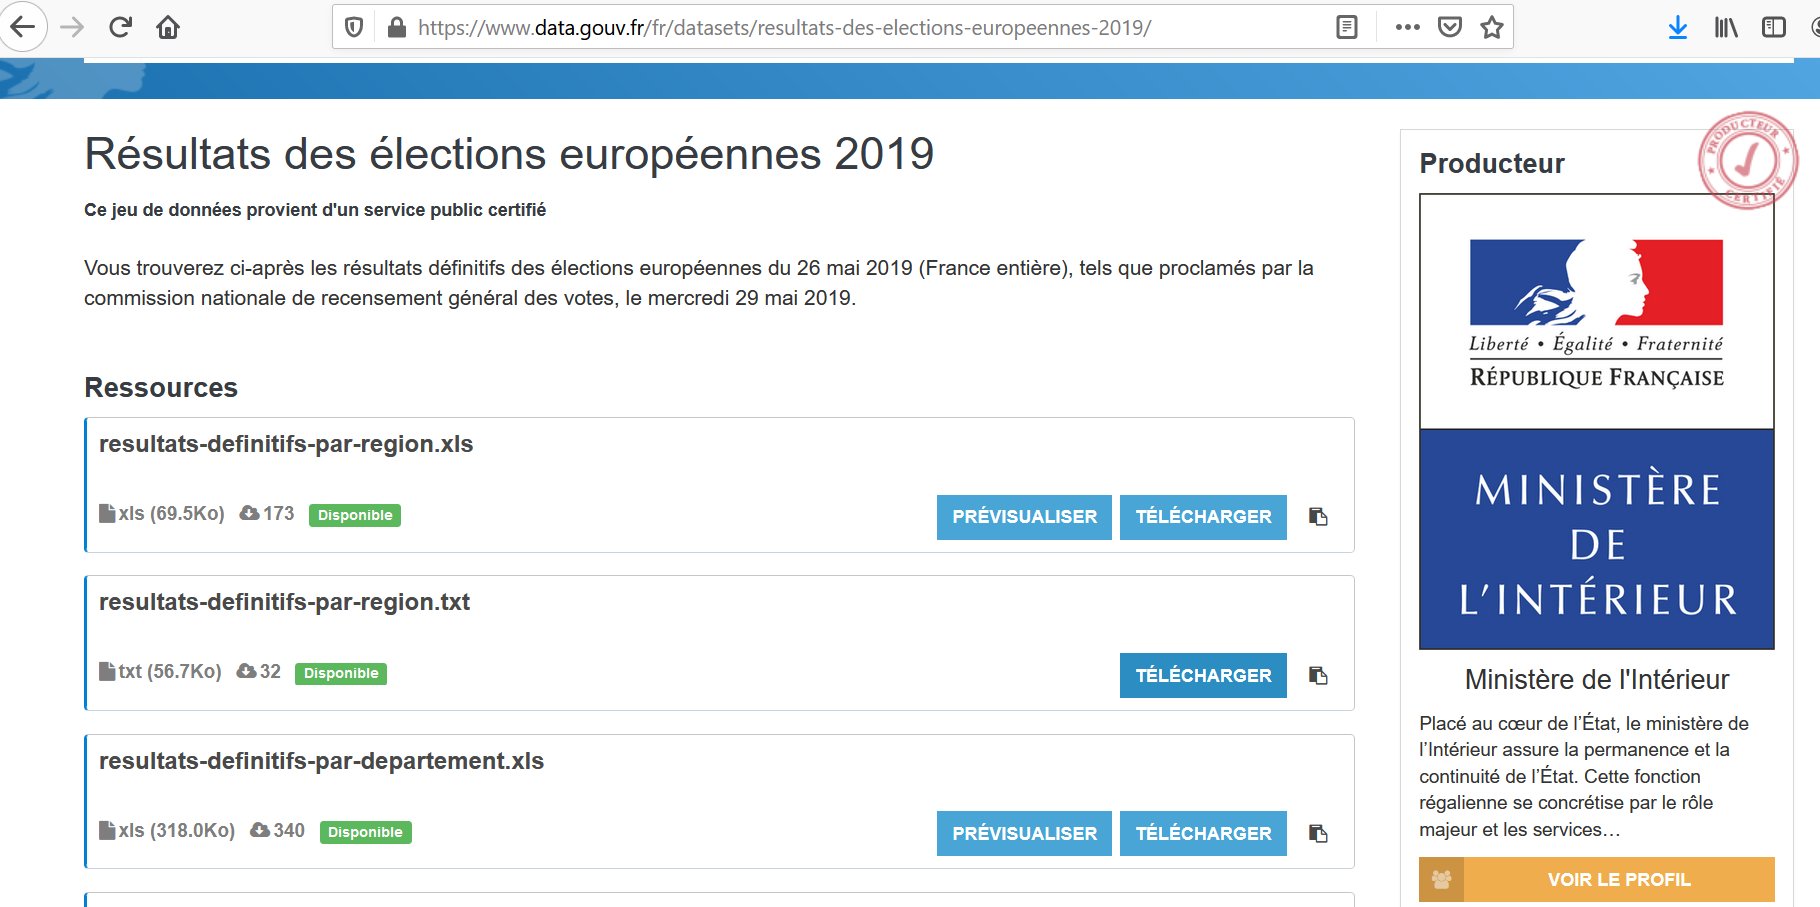
\includegraphics[width=0.75\textwidth,height=\textheight]{fig/datagouvMI.png}
\caption{Portail du ministère de l'intérieur sur data.gouv.fr}
\end{figure}

\hypertarget{remarques-sur-la-structure-des-donnuxe9es}{%
\subsubsection{Remarques sur la structure des
données}\label{remarques-sur-la-structure-des-donnuxe9es}}

Quand on télécharge les résultats sous format Excel, on découvre qu'un
certain nombre de colonnes du tableau ne comporte pas de noms à la 1ère
du fichier. Il s'agit des noms des colonnes pour les listes n°2 et
suivantes des candidatures en lice. Les colonnes du tableau n'ont pas
toujours de noms en en-tête de fichier. Dans l'exemple ci-dessous des
résultats des élections européennes en 2019 au niveau des départements,
toutes les colonnes de A à W ont un nom d'en-tête, les suivantes n'ont
pas de nom.

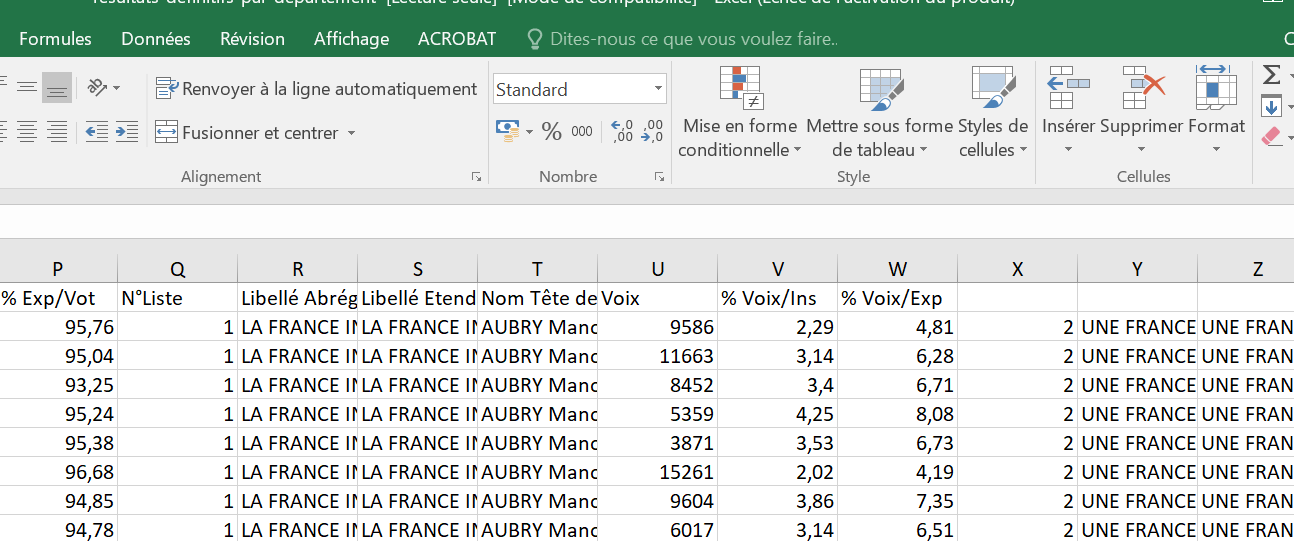
\includegraphics[width=0.75\textwidth,height=\textheight]{fig/resultats-excel.png}

Le fichier tel qu'il est construit n'est pas directement exploitable
pour des traitements statistiques ou cartographiques par exemple. Le
tableau est de largeur variable pour chaque ligne du jeu de données. En
règle générale, comme l'offre électorale dans un échelon géographique
donné diffère presque toujours d'un autre échelon, il en résulte que le
tableau n'a pas les mêmes champs de l'offre électorale d'une ligne à
l'autre. Donc, chaque ligne du tableau a un nombre variable
d'informations données sur les listes des candidats et leurs scores
obtenus.

Il n'est pas immédiat de pouvoir effectuer des opérations arithmétiques
sur les nombres de voix obtenues par les différentes listes de candidats
sur un tel fichier. C'est pourquoi il faut transformer ce fichier en un
tableau sous forme de matrice des voix pour chaque nuance politique qui
soit uniforme pour toutes lignes du tableau.

\hypertarget{transformer-le-fichier-uxe0-laide-de-lapplication-lireinteractif}{%
\section{\texorpdfstring{Transformer le fichier à l'aide de
l'application
\texttt{LireInteractif}}{Transformer le fichier à l'aide de l'application LireInteractif}}\label{transformer-le-fichier-uxe0-laide-de-lapplication-lireinteractif}}

\hypertarget{introduction-du-package-liremininterieur}{%
\subsection{\texorpdfstring{Introduction du package
\texttt{LireMinInterieur}}{Introduction du package LireMinInterieur}}\label{introduction-du-package-liremininterieur}}

Le politologue Joël Gombin a developpé le package
\href{https://github.com/joelgombin/LireMinInterieur}{LireMinInterieur},
disponible non pas sur le CRAN mais sur le dépôt Github\footnote{\url{https://github.com/joelgombin/LireMinInterieur}}
de l'auteur, qui propose un outil très utile pour nettoyer et mettre en
forme les résultats électoraux du Ministère de l'Intérieur.

On l'installe depuis la console R avec la commande :

\begin{Shaded}
\begin{Highlighting}[]
\FunctionTok{library}\NormalTok{(devtools)}
\FunctionTok{install\_github}\NormalTok{(}\StringTok{"joelgombin/LireMinInterieur"}\NormalTok{)}
\end{Highlighting}
\end{Shaded}

\hypertarget{application-lireinteractif}{%
\subsection{\texorpdfstring{Application
\texttt{LireInteractif}}{Application LireInteractif}}\label{application-lireinteractif}}

Il existe une application développée dans \texttt{Shiny} pour
transformer les fichiers du Ministère, c'est \texttt{LireInteractif}. On
charge en mémoire le package \texttt{LireMinInterieur} et on lance
l'application par la commande :

\begin{Shaded}
\begin{Highlighting}[]
\FunctionTok{library}\NormalTok{(LireMinInterieur)}
\FunctionTok{lireInteractif}\NormalTok{()}
\end{Highlighting}
\end{Shaded}

Dans la fenêtre de l'application, on peut voir dans le panneau de gauche
les informations entrées par l'utilisateur et dans celui de droite une
vue du fichier électoral avant et après sa transformation.

\begin{figure}

{\centering 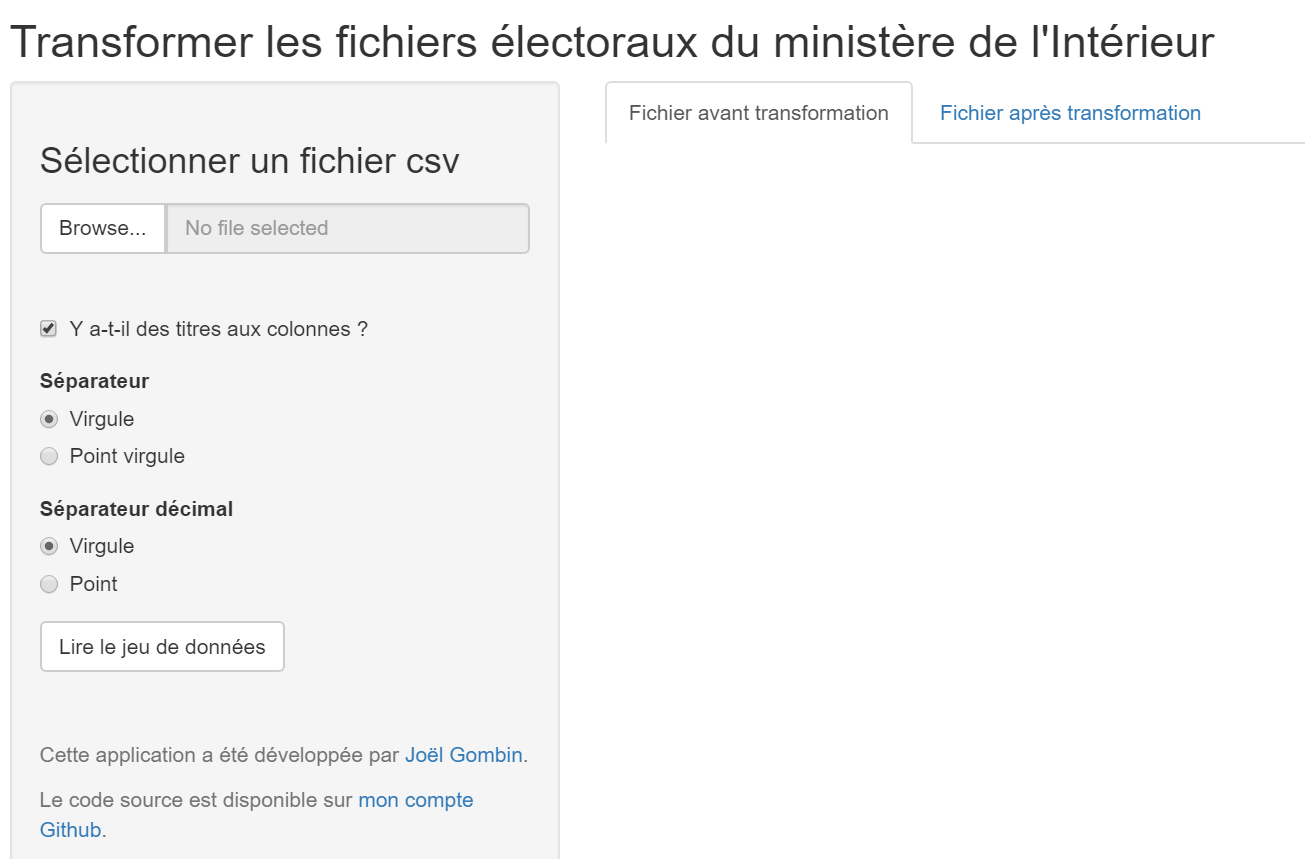
\includegraphics[width=0.75\linewidth]{fig/capture_lireInteractive} 

}

\caption{Aperçu de l'application lireInteractif}\label{fig:apercu_api}
\end{figure}

\hypertarget{import-du-tableau-uxe0-transformer}{%
\subsubsection{Import du tableau à
transformer}\label{import-du-tableau-uxe0-transformer}}

Dans le panneau de gauche, l'utilisateur indique d'abord charge le
fichier .csv qu'il veut transformer en précisant le type de séparateur
de colonnes (par défaut la virgule) et le séparateur décimal (par défaut
la virgule). Le chargement du fichier est bien effectué à cette étape
quand le message ``Upload complete'' est affché\footnote{Veiller à ce
  que la taille du fichier à lire ne dépasse pas la limite maximale de
  chargement de fixée fixée à 100 Mo. Cette limite peut être modifiée
  dans les options de Shiny,
  options(shiny.maxRequestSize=\textbf{100}*1024\^{}2)}. Ensuite quand
l'utilisateur clique sur le bouton \texttt{Lire\ le\ jeu\ de\ données},
le panneau de droite affiche le fichier importé avant sa transformation.

\begin{figure}

{\centering 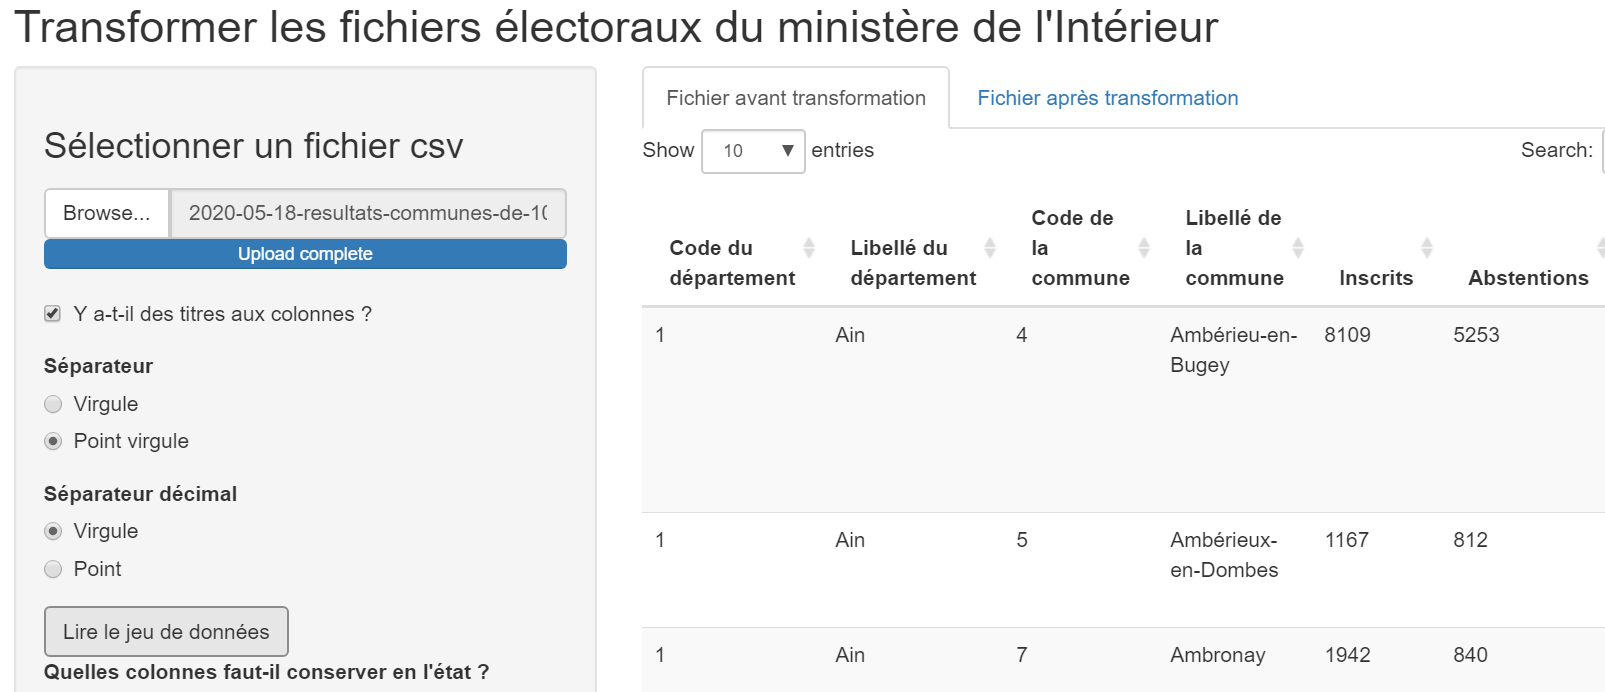
\includegraphics[width=0.75\linewidth]{fig/import_file_csv} 

}

\caption{Import du fichier à transformer}\label{fig:load_file}
\end{figure}

Après avoir lu le fichier, il apparaît une nouvelle zone de paramètres à
renseigner dans le panneau de droite. Cette zone requiert les
informations suivantes :

\begin{itemize}
\tightlist
\item
  les colonnes à conserver dans le fichier en l'état. Choisir dans le
  menu déroulant les noms des colonnes que l'on souhaite conserver dans
  le fichier transformer ;
\item
  les nouveaux noms à attribuer aux colonnes choisies (accepter par
  défaut les noms proposés). A minima les colonnes \emph{Inscrits} et
  \emph{Exprimés} sont requises ;
\item
  la première colonne du fichier qui contient le code nuance politique ;
\item
  le nombre de colonnes situées entre les colonnes contenant le code
  nuance politique (par défaut 7) ;
\item
  le nombre de colonnes du fichier qui séparent les colonnes avec les
  nuances politiques et les colonnes avec le nombre de suffrages
  exprimés (par défaut 3)
\end{itemize}

\begin{figure}

{\centering 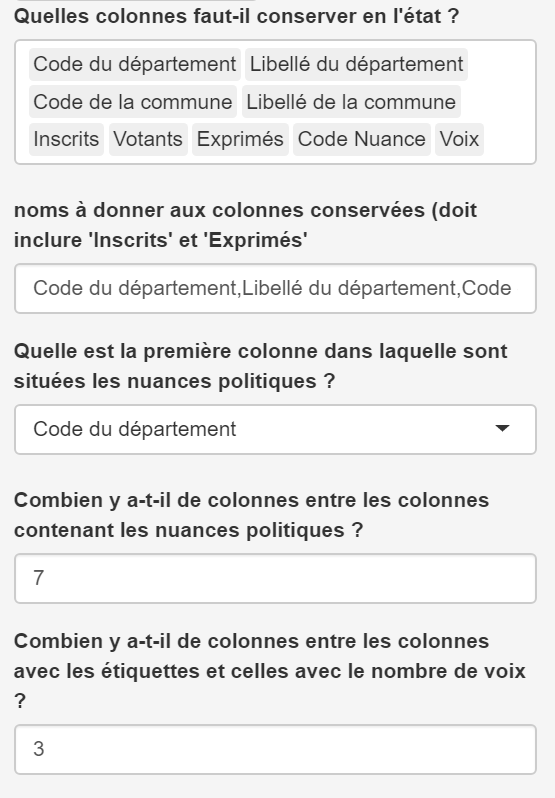
\includegraphics[width=0.3\linewidth]{fig/avant_transformation} 

}

\caption{Paramètres pour la transformation du fichier}\label{fig:avant_transfo}
\end{figure}

Enfin, l'utilisateur peut appuyer sur le bonton
\texttt{Transformer\ le\ fichier} situé en bas du panneau pour afficher
dans le panneau de droite le fichier transformé.

\begin{figure}

{\centering 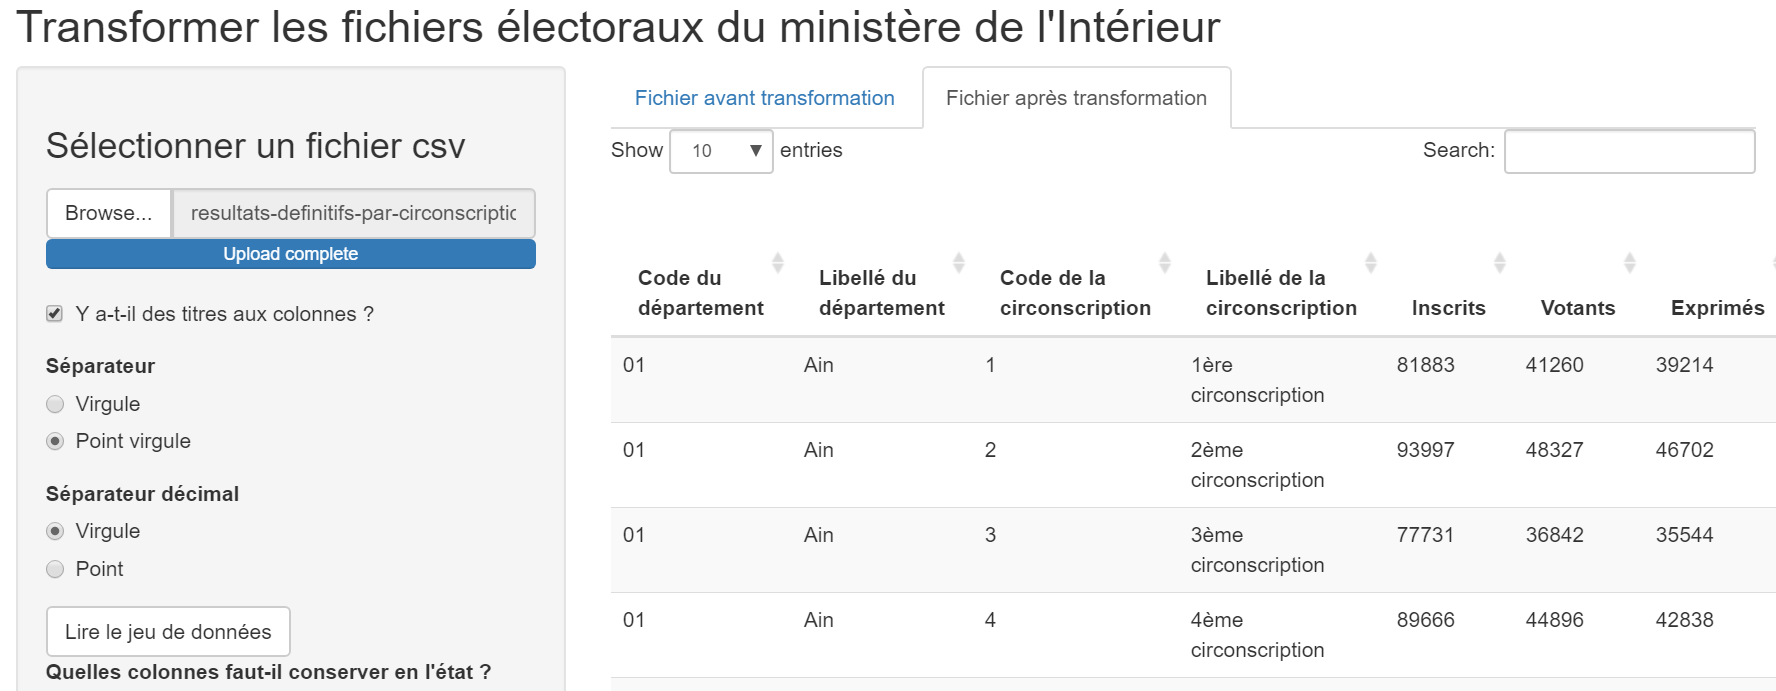
\includegraphics[width=0.75\linewidth]{fig/apres_transformation} 

}

\caption{Affichage du fichier après transformation}\label{fig:apres_transfo}
\end{figure}

\hypertarget{export-du-tableau-transformuxe9}{%
\subsubsection{Export du tableau
transformé}\label{export-du-tableau-transformuxe9}}

L'utilisateur peut télécharger le fichier transformé en cliquant sur le
bouton \texttt{Télécharger} situé en bas à gauche du panneau de droite
sous le fichier. Le fichier est téléchargé sous le répertoire indiqué
par l'utilisateur au format CSV.

\begin{figure}

{\centering 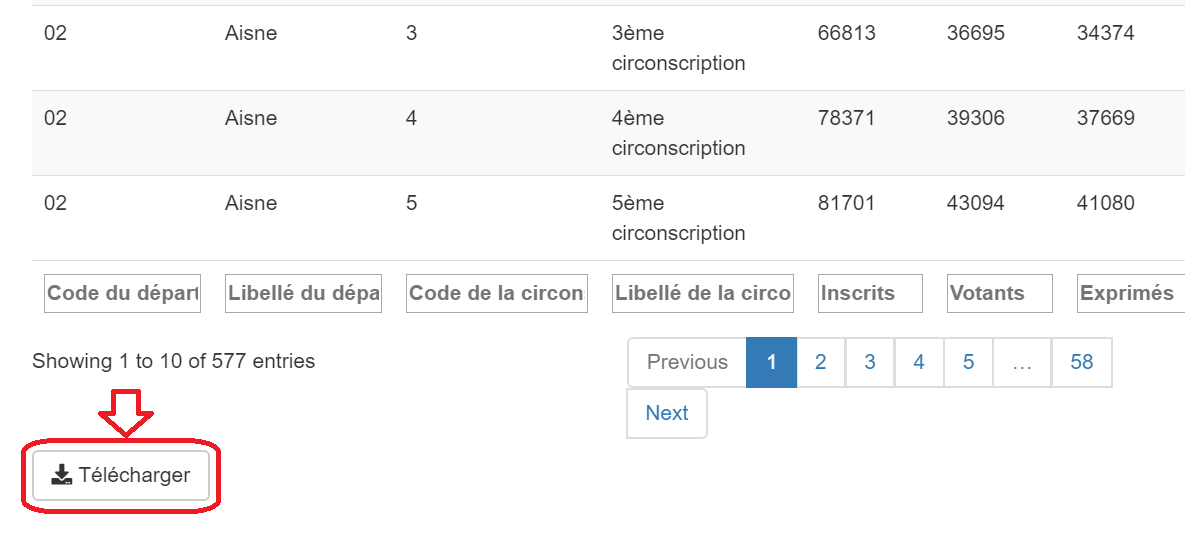
\includegraphics[width=0.75\linewidth]{fig/telecharger_apres_transformation} 

}

\caption{Télécharger le fichier transformé}\label{fig:telecharger}
\end{figure}

\hypertarget{lecture-du-fichier-dans-un-tableur}{%
\subsubsection{Lecture du fichier dans un
tableur}\label{lecture-du-fichier-dans-un-tableur}}

Pour ouvrir ce fichier CSV par exemple dans un tableur Excel, on déclare
les colonnes du fichier et on choisit lesquelles on conserve dans le
menu \texttt{Données\textbackslash{}Convertir} de Excel. Ensuite, avec
l'aide de l'assistant conversion, on peut sélectionner comment sont
stockées les données dans le fichier :

\begin{itemize}
\tightlist
\item
  Délimité (les colonnes du fichier sont séparés par un caractère
  spécial, la virgule, le point-virgule, etc.), c'est cette option qui
  est retenue ;
\item
  Largeur fixe (les champs sont rangées en colonne de largeur fixe et
  séparés par des espace)
\end{itemize}

\begin{center}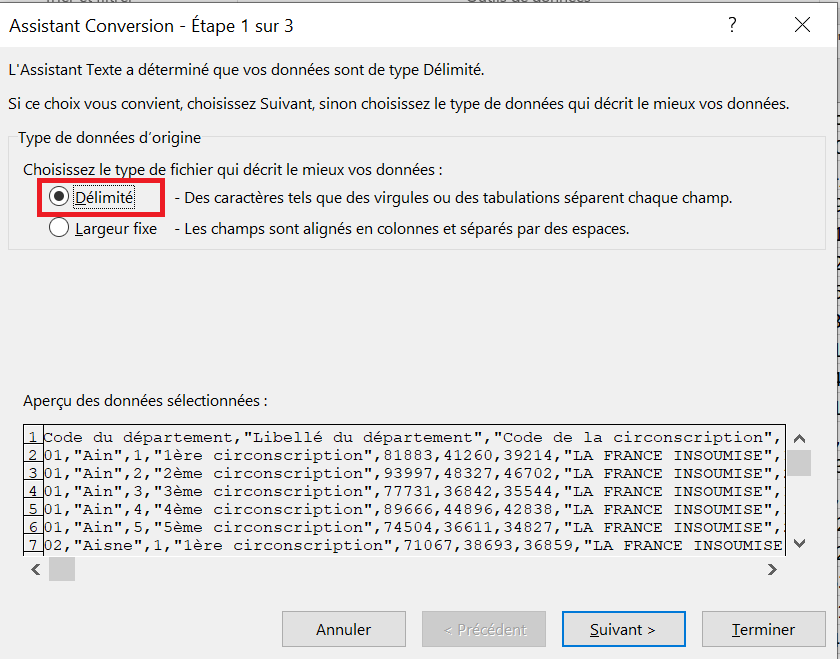
\includegraphics[width=0.5\linewidth]{fig/assistant_conversion_1_3} \end{center}

Ensuite, après avoir choisi l'option délimité à l'étape 1, il faut
indiquer quel est le type de séparateur de colonnes du fichier CSV. On
coche le séparateur de la virgule et on clique sur le bouton suivant.

\begin{center}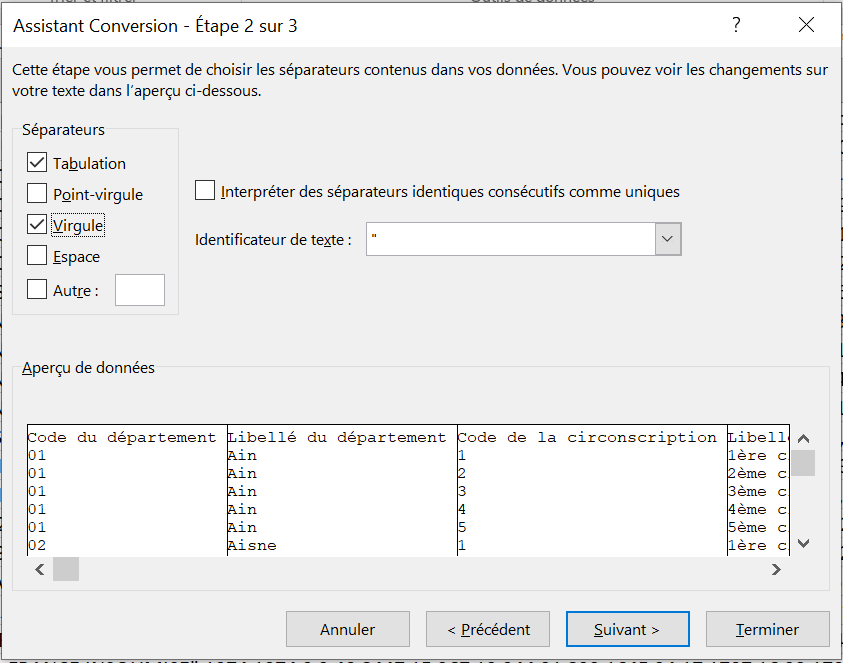
\includegraphics[width=0.5\linewidth]{fig/assistant_conversion_2_3} \end{center}

A la dernière étape, on peut choisir dans quel format sont converties
les données du fichier. Les formats possibles de lecture/conversion des
données sont le format standard, le format texte, le format date. Il est
aussi possible de choisir de ne pas retenir telle ou telle colonne en
sélectionnant l'option \texttt{colonne\ non\ distribuée}. Ici, on
accepte les formats choisis par défaut et on clique sur le bouton
\texttt{Terminer}.

\begin{center}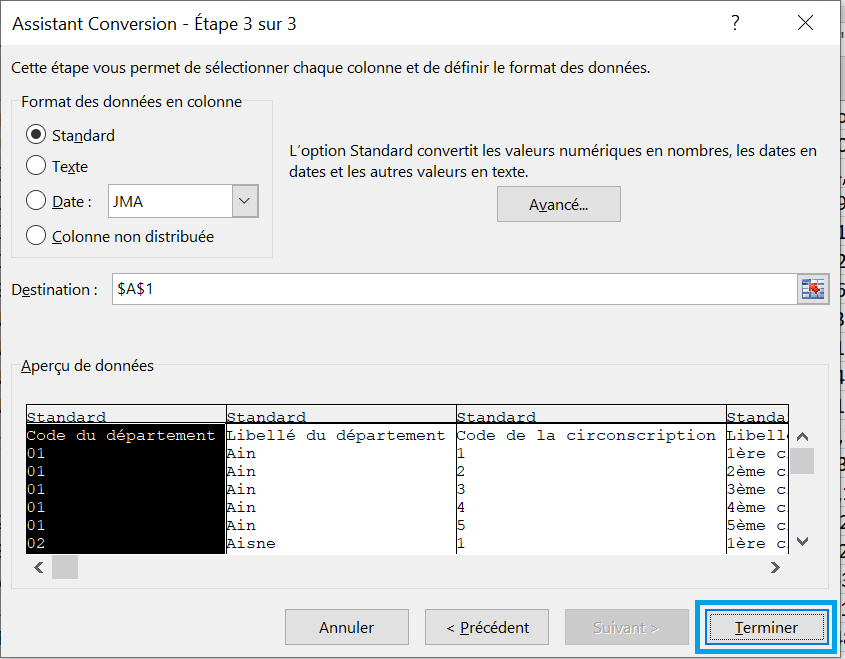
\includegraphics[width=0.5\linewidth]{fig/assistant_conversion_3_3} \end{center}

On obtient le fichier transformé en matrice des voix exporté dans Excel
pour d'autres calculs.

\begin{figure}
\centering
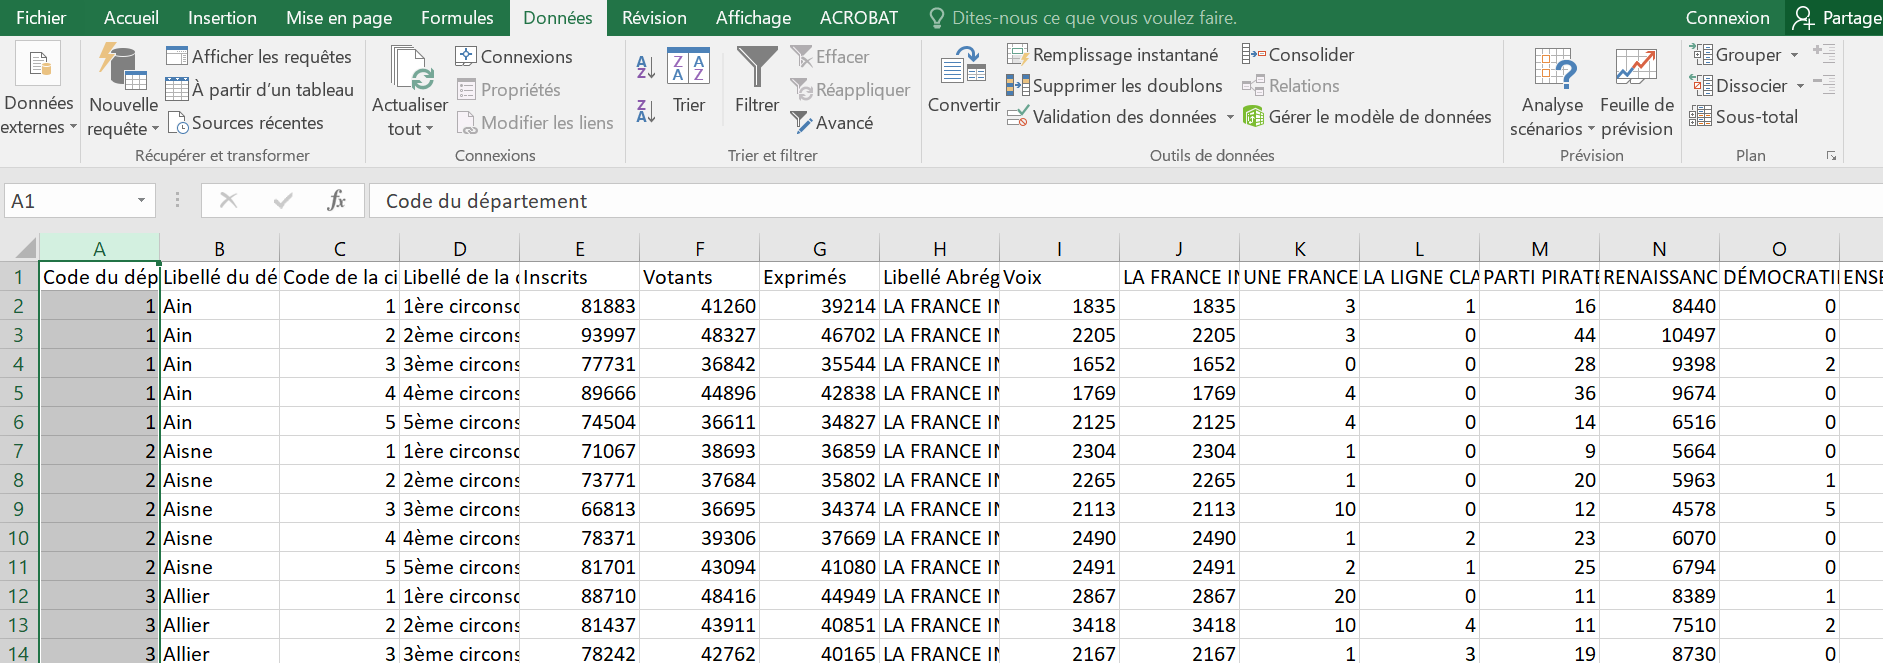
\includegraphics{fig/tableau_matrice_des_voix.PNG}
\caption{Affichage du tableau tranformé par l'API LireInterieur et
exporté dans Excel}
\end{figure}

\hypertarget{annexe}{%
\section{Annexe}\label{annexe}}

\hypertarget{la-fonction-lire}{%
\subsection{\texorpdfstring{La fonction
\texttt{lire}}{La fonction lire}}\label{la-fonction-lire}}

Pour aller plus loin, il peut être utile de connaître la fonction
\texttt{lire} qui est à la base de la transformation des fichiers
électoraux du Ministère de l'Intérieur.

La fonction \texttt{lire} est utile pour transformer les fichiers de
résultats électoraux diffusés par le ministère de l'Intérieur français,
lorsque l'offre électorale n'est pas homogène sur l'ensemble du
territoire (législatives, européennes, cantonales, régionales\ldots).
Pour ce faire, les résultats sont agrégés en fonction des étiquettes
attribuées par le ministère de l'intérieur.

Cette fonction est définie avec les 5 arguments suivants :

\begin{itemize}
\tightlist
\item
  \emph{X}, le data.frame d'origine importé depuis un fichier plat CSV
  généralement ;
\item
  \emph{keep}, un vecteur indiquant les numéros (ou les noms) des
  colonnes de X qui sont à conserver telles quelles. Les colonnes
  Inscrits et Exprimés sont requises ;
\item
  \emph{col}, un vecteur indiquant le numéro des colonnes contenant les
  étiquettes de nuances politiques à partir desquelles les résultats
  sont agrégés. En général, leur espacement est régulier et peut
  s'écrire sous la forme d'une séquence de nombres seq(10, 100, 10) ;
\item
  \emph{keep.names}, le nom à donner aux colonnes retenues. Par défaut,
  c'est le nom d'origine des colonnes ;
\item
  \emph{gap}, le nombre de colonnes intercalées entre la colonne des
  étiquettes et celle du nombre de voix. Par défaut 3
\end{itemize}

\end{document}
